\documentclass[border=2pt]{standalone}
\usepackage{tikz}
\usetikzlibrary{arrows.meta,chains}

\begin{document}
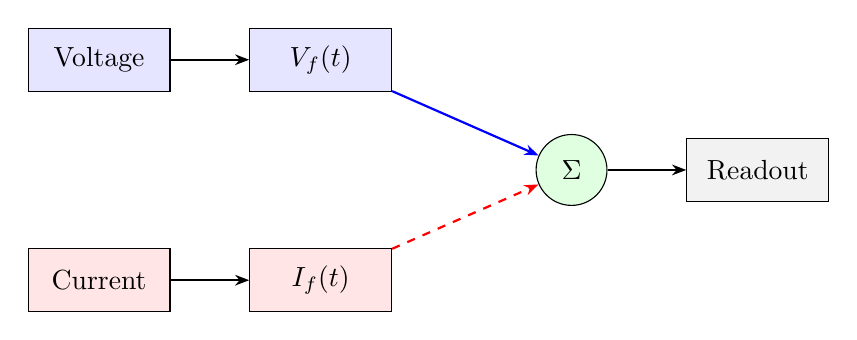
\begin{tikzpicture}[
  node distance=5mm and 10mm,
  start chain=voltage going right,
  start chain=current going right,
  start chain=readout going right,
  block/.style={draw,minimum width=18mm,minimum height=8mm,align=center},
  every on chain/.style={join},
  every join/.style={-{Stealth[length=1.8mm]},thick}
]
  \node[block,on chain=voltage,fill=blue!10] (voltage-sensor) at (0,1.4) {Voltage};
  \node[block,on chain=voltage,fill=blue!10] (voltage-filter) {$V_f(t)$};

  \node[block,on chain=current,fill=red!10] (current-sensor) at (0,-1.4) {Current};
  \node[block,on chain=current,fill=red!10] (current-filter) {$I_f(t)$};

  \node[
    draw,
    circle,
    minimum size=9mm,
    on chain=readout,
    fill=green!12,
    join=with voltage-end by {blue},
    join=with current-end by {red,dashed}
  ] (mixer) at (6,0) {$\Sigma$};
  \node[block,on chain=readout,fill=gray!10] (scope) {Readout};
\end{tikzpicture}
\end{document}
